%  LaTeX support: latex@mdpi.com
%  For support, please attach all files needed for compiling as well as the log file, and specify your operating system, LaTeX version, and LaTeX editor.

%=================================================================
% pandoc conditionals added to preserve backwards compatibility with previous versions of rticles

\documentclass[notspecified,article,submit,moreauthors,pdftex]{Definitions/mdpi}


%% Some pieces required from the pandoc template
\setlist[itemize]{leftmargin=*,labelsep=5.8mm}
\setlist[enumerate]{leftmargin=*,labelsep=4.9mm}


%--------------------
% Class Options:
%--------------------

%---------
% article
%---------
% The default type of manuscript is "article", but can be replaced by:
% abstract, addendum, article, book, bookreview, briefreport, casereport, comment, commentary, communication, conferenceproceedings, correction, conferencereport, entry, expressionofconcern, extendedabstract, datadescriptor, editorial, essay, erratum, hypothesis, interestingimage, obituary, opinion, projectreport, reply, retraction, review, perspective, protocol, shortnote, studyprotocol, systematicreview, supfile, technicalnote, viewpoint, guidelines, registeredreport, tutorial
% supfile = supplementary materials

%----------
% submit
%----------
% The class option "submit" will be changed to "accept" by the Editorial Office when the paper is accepted. This will only make changes to the frontpage (e.g., the logo of the journal will get visible), the headings, and the copyright information. Also, line numbering will be removed. Journal info and pagination for accepted papers will also be assigned by the Editorial Office.

%------------------
% moreauthors
%------------------
% If there is only one author the class option oneauthor should be used. Otherwise use the class option moreauthors.

%---------
% pdftex
%---------
% The option pdftex is for use with pdfLaTeX. Remove "pdftex" for (1) compiling with LaTeX & dvi2pdf (if eps figures are used) or for (2) compiling with XeLaTeX.

%=================================================================
% MDPI internal commands - do not modify
\firstpage{1}
\makeatletter
\setcounter{page}{\@firstpage}
\makeatother
\pubvolume{1}
\issuenum{1}
\articlenumber{0}
\pubyear{2023}
\copyrightyear{2023}
%\externaleditor{Academic Editor: Firstname Lastname}
\datereceived{ }
\daterevised{ } % Comment out if no revised date
\dateaccepted{ }
\datepublished{ }
%\datecorrected{} % For corrected papers: "Corrected: XXX" date in the original paper.
%\dateretracted{} % For corrected papers: "Retracted: XXX" date in the original paper.
\hreflink{https://doi.org/} % If needed use \linebreak
%\doinum{}
%\pdfoutput=1 % Uncommented for upload to arXiv.org

%=================================================================
% Add packages and commands here. The following packages are loaded in our class file: fontenc, inputenc, calc, indentfirst, fancyhdr, graphicx, epstopdf, lastpage, ifthen, float, amsmath, amssymb, lineno, setspace, enumitem, mathpazo, booktabs, titlesec, etoolbox, tabto, xcolor, colortbl, soul, multirow, microtype, tikz, totcount, changepage, attrib, upgreek, array, tabularx, pbox, ragged2e, tocloft, marginnote, marginfix, enotez, amsthm, natbib, hyperref, cleveref, scrextend, url, geometry, newfloat, caption, draftwatermark, seqsplit
% cleveref: load \crefname definitions after \begin{document}

%=================================================================
% Please use the following mathematics environments: Theorem, Lemma, Corollary, Proposition, Characterization, Property, Problem, Example, ExamplesandDefinitions, Hypothesis, Remark, Definition, Notation, Assumption
%% For proofs, please use the proof environment (the amsthm package is loaded by the MDPI class).

%=================================================================
% Full title of the paper (Capitalized)
\Title{Full title of the paper (Capitalized)}

% MDPI internal command: Title for citation in the left column
\TitleCitation{Full title of the paper (Capitalized)}

% Author Orchid ID: enter ID or remove command
%\newcommand{\orcidauthorA}{0000-0000-0000-000X} % Add \orcidA{} behind the author's name
%\newcommand{\orcidauthorB}{0000-0000-0000-000X} % Add \orcidB{} behind the author's name


% Authors, for the paper (add full first names)
\Author{Sara Marquínez Díaz$^{1}$, Ángel Lapeña López$^{1}$, Javier
Rodríguez Jiménez$^{1}$}


%\longauthorlist{yes}


% MDPI internal command: Authors, for metadata in PDF
\AuthorNames{Sara Marquínez Díaz, Ángel Lapeña López, Javier Rodríguez
Jiménez}

% MDPI internal command: Authors, for citation in the left column

% Affiliations / Addresses (Add [1] after \address if there is only one affiliation.)
\address{%
$^{1}$ \quad Máster Universitario en Ciencia de Datos - Universitat de
València.; \\
}

% Contact information of the corresponding author
\corres{Correspondence: \href{mailto:marquin9@alumni.uv.es}{\nolinkurl{marquin9@alumni.uv.es}},
\href{mailto:anlalo2@alumni.uv.es}{\nolinkurl{anlalo2@alumni.uv.es}},
\href{mailto:jaroji@alumni.uv.es}{\nolinkurl{jaroji@alumni.uv.es}}}

% Current address and/or shared authorship








% The commands \thirdnote{} till \eighthnote{} are available for further notes

% Simple summary
\simplesumm{A Simple summary goes here.}

%\conference{} % An extended version of a conference paper

% Abstract (Do not insert blank lines, i.e. \\)
\abstract{A single paragraph of about 200 words maximum. For research
articles, abstracts should give a pertinent overview of the work. We
strongly encourage authors to use the following style of structured
abstracts, but without The abstract should be an objective
representation of the article, it must not contain results which are not
presented and substantiated in the main text and should not exaggerate
the main conclusions. headings: 1) Background: Place the question
addressed in a broad context and highlight the purpose of the study; 2)
Methods: Describe briefly the main methods or treatments applied; 3)
Results: Summarize the article's main findings; and 4) Conclusion:
Indicate the main conclusions or interpretations.}


% Keywords
\keyword{keyword 1; keyword 2; keyword 3 (list three to ten pertinent
keywords specific to the article, yet reasonably common within the
subject discipline.).}

% The fields PACS, MSC, and JEL may be left empty or commented out if not applicable
%\PACS{J0101}
%\MSC{}
%\JEL{}

%%%%%%%%%%%%%%%%%%%%%%%%%%%%%%%%%%%%%%%%%%
% Only for the journal Diversity
%\LSID{\url{http://}}

%%%%%%%%%%%%%%%%%%%%%%%%%%%%%%%%%%%%%%%%%%
% Only for the journal Applied Sciences

%%%%%%%%%%%%%%%%%%%%%%%%%%%%%%%%%%%%%%%%%%

%%%%%%%%%%%%%%%%%%%%%%%%%%%%%%%%%%%%%%%%%%
% Only for the journal Data



%%%%%%%%%%%%%%%%%%%%%%%%%%%%%%%%%%%%%%%%%%
% Only for the journal Toxins


%%%%%%%%%%%%%%%%%%%%%%%%%%%%%%%%%%%%%%%%%%
% Only for the journal Encyclopedia


%%%%%%%%%%%%%%%%%%%%%%%%%%%%%%%%%%%%%%%%%%
% Only for the journal Advances in Respiratory Medicine
%\addhighlights{yes}
%\renewcommand{\addhighlights}{%

%\noindent This is an obligatory section in “Advances in Respiratory Medicine”, whose goal is to increase the discoverability and readability of the article via search engines and other scholars. Highlights should not be a copy of the abstract, but a simple text allowing the reader to quickly and simplified find out what the article is about and what can be cited from it. Each of these parts should be devoted up to 2~bullet points.\vspace{3pt}\\
%\textbf{What are the main findings?}
% \begin{itemize}[labelsep=2.5mm,topsep=-3pt]
% \item First bullet.
% \item Second bullet.
% \end{itemize}\vspace{3pt}
%\textbf{What is the implication of the main finding?}
% \begin{itemize}[labelsep=2.5mm,topsep=-3pt]
% \item First bullet.
% \item Second bullet.
% \end{itemize}
%}


%%%%%%%%%%%%%%%%%%%%%%%%%%%%%%%%%%%%%%%%%%

% Pandoc syntax highlighting
\usepackage{color}
\usepackage{fancyvrb}
\newcommand{\VerbBar}{|}
\newcommand{\VERB}{\Verb[commandchars=\\\{\}]}
\DefineVerbatimEnvironment{Highlighting}{Verbatim}{commandchars=\\\{\}}
% Add ',fontsize=\small' for more characters per line
\usepackage{framed}
\definecolor{shadecolor}{RGB}{248,248,248}
\newenvironment{Shaded}{\begin{snugshade}}{\end{snugshade}}
\newcommand{\AlertTok}[1]{\textcolor[rgb]{0.94,0.16,0.16}{#1}}
\newcommand{\AnnotationTok}[1]{\textcolor[rgb]{0.56,0.35,0.01}{\textbf{\textit{#1}}}}
\newcommand{\AttributeTok}[1]{\textcolor[rgb]{0.13,0.29,0.53}{#1}}
\newcommand{\BaseNTok}[1]{\textcolor[rgb]{0.00,0.00,0.81}{#1}}
\newcommand{\BuiltInTok}[1]{#1}
\newcommand{\CharTok}[1]{\textcolor[rgb]{0.31,0.60,0.02}{#1}}
\newcommand{\CommentTok}[1]{\textcolor[rgb]{0.56,0.35,0.01}{\textit{#1}}}
\newcommand{\CommentVarTok}[1]{\textcolor[rgb]{0.56,0.35,0.01}{\textbf{\textit{#1}}}}
\newcommand{\ConstantTok}[1]{\textcolor[rgb]{0.56,0.35,0.01}{#1}}
\newcommand{\ControlFlowTok}[1]{\textcolor[rgb]{0.13,0.29,0.53}{\textbf{#1}}}
\newcommand{\DataTypeTok}[1]{\textcolor[rgb]{0.13,0.29,0.53}{#1}}
\newcommand{\DecValTok}[1]{\textcolor[rgb]{0.00,0.00,0.81}{#1}}
\newcommand{\DocumentationTok}[1]{\textcolor[rgb]{0.56,0.35,0.01}{\textbf{\textit{#1}}}}
\newcommand{\ErrorTok}[1]{\textcolor[rgb]{0.64,0.00,0.00}{\textbf{#1}}}
\newcommand{\ExtensionTok}[1]{#1}
\newcommand{\FloatTok}[1]{\textcolor[rgb]{0.00,0.00,0.81}{#1}}
\newcommand{\FunctionTok}[1]{\textcolor[rgb]{0.13,0.29,0.53}{\textbf{#1}}}
\newcommand{\ImportTok}[1]{#1}
\newcommand{\InformationTok}[1]{\textcolor[rgb]{0.56,0.35,0.01}{\textbf{\textit{#1}}}}
\newcommand{\KeywordTok}[1]{\textcolor[rgb]{0.13,0.29,0.53}{\textbf{#1}}}
\newcommand{\NormalTok}[1]{#1}
\newcommand{\OperatorTok}[1]{\textcolor[rgb]{0.81,0.36,0.00}{\textbf{#1}}}
\newcommand{\OtherTok}[1]{\textcolor[rgb]{0.56,0.35,0.01}{#1}}
\newcommand{\PreprocessorTok}[1]{\textcolor[rgb]{0.56,0.35,0.01}{\textit{#1}}}
\newcommand{\RegionMarkerTok}[1]{#1}
\newcommand{\SpecialCharTok}[1]{\textcolor[rgb]{0.81,0.36,0.00}{\textbf{#1}}}
\newcommand{\SpecialStringTok}[1]{\textcolor[rgb]{0.31,0.60,0.02}{#1}}
\newcommand{\StringTok}[1]{\textcolor[rgb]{0.31,0.60,0.02}{#1}}
\newcommand{\VariableTok}[1]{\textcolor[rgb]{0.00,0.00,0.00}{#1}}
\newcommand{\VerbatimStringTok}[1]{\textcolor[rgb]{0.31,0.60,0.02}{#1}}
\newcommand{\WarningTok}[1]{\textcolor[rgb]{0.56,0.35,0.01}{\textbf{\textit{#1}}}}

% tightlist command for lists without linebreak
\providecommand{\tightlist}{%
  \setlength{\itemsep}{0pt}\setlength{\parskip}{0pt}}



\usepackage{longtable}

\begin{document}



%%%%%%%%%%%%%%%%%%%%%%%%%%%%%%%%%%%%%%%%%%

\newcommand{\pandocbounded}[1]{#1}

\section{Version}\label{version}

This Rmd-skeleton uses the mdpi Latex template published 2023-03-25.
However, the official template gets more frequently updated than the
\textbf{rticles} package. Therefore, please make sure prior to paper
submission, that you're using the most recent .cls, .tex and .bst files
(available \href{http://www.mdpi.com/authors/latex}{here}).

\section{Article Header Information}\label{article-header-information}

The YAML header includes information needed mainly for formatting the
front and back matter of the article. Required elements include:

\begin{Shaded}
\begin{Highlighting}[]
\FunctionTok{title}\KeywordTok{:}\AttributeTok{ Title of the paper}
\FunctionTok{author}\KeywordTok{:}
\AttributeTok{  }\KeywordTok{{-}}\AttributeTok{ }\FunctionTok{name}\KeywordTok{:}\AttributeTok{ first and last name}
\FunctionTok{    affil}\KeywordTok{: }\CharTok{|}
\NormalTok{      One or more comma seperated numbers corresponding to affilitation}
\NormalTok{      and one or more  comma seperated symbols corresponding }
\NormalTok{      optional notes.}
\AttributeTok{    }\FunctionTok{orcid}\KeywordTok{:}\AttributeTok{ optional orcid number}
\FunctionTok{affiliation}\KeywordTok{:}\AttributeTok{  }
\AttributeTok{  }\KeywordTok{{-}}\AttributeTok{ }\FunctionTok{num}\KeywordTok{:}\AttributeTok{ 1,..., n for each affiliation}
\AttributeTok{    }\FunctionTok{address}\KeywordTok{:}\AttributeTok{ required}
\AttributeTok{    }\FunctionTok{email}\KeywordTok{:}\AttributeTok{ required}
\FunctionTok{authorcitation}\KeywordTok{: }\CharTok{|}
\NormalTok{  Lastname, F.}
\FunctionTok{correspondence}\KeywordTok{: }\CharTok{|}
\NormalTok{  email@email.com; Tel.: +XX{-}000{-}00{-}0000.}
\FunctionTok{journal}\KeywordTok{:}\AttributeTok{ notspecified}
\FunctionTok{type}\KeywordTok{:}\AttributeTok{ article}
\FunctionTok{status}\KeywordTok{:}\AttributeTok{ submit}
\end{Highlighting}
\end{Shaded}

Journal options are in Table \ref{tab:mdpinames}. The \texttt{status}
variable should generally not be changed by authors. The \texttt{type}
variable describes the type of of submission and defaults to
\texttt{article} but can be replaced with any of the ones in Table
\ref{tab:mdpitype}

\begin{table}

\caption{\label{tab:mdpitype}MDPI article types.}
\centering
\begin{tabular}[t]{lll}
\toprule
abstract & entry & retraction\\
addendum & expressionofconcern & review\\
article & extendedabstract & perspective\\
book & datadescriptor & protocol\\
bookreview & editorial & shortnote\\
\addlinespace
briefreport & essay & studyprotocol\\
casereport & erratum & systematicreview\\
comment & hypothesis & supfile\\
commentary & interestingimage & technicalnote\\
communication & obituary & viewpoint\\
\addlinespace
conferenceproceedings & opinion & guidelines\\
correction & projectreport & registeredreport\\
conferencereport & reply & tutorial\\
\bottomrule
\end{tabular}
\end{table}

\subsection{Journal Specific YAML
variables}\label{journal-specific-yaml-variables}

\begin{Shaded}
\begin{Highlighting}[]
\CommentTok{\# for journal Diversity,}
\CommentTok{\# add the Life Science Identifier using:}
\FunctionTok{lsid}\KeywordTok{:}\AttributeTok{ http://zoobank.org/urn:lsid:zoobank.org:act:nnnn}


\CommentTok{\# for journal Applied Sciences}
\CommentTok{\# add featured application}
\FunctionTok{featuredapplication}\KeywordTok{: }\CharTok{|}
\NormalTok{  Authors are encouraged to provide a concise }
\NormalTok{  description of the specific application or }
\NormalTok{  a potential application of the work. This }
\NormalTok{  section is not mandatory.}

\CommentTok{\# for the journal Data}
\CommentTok{\# add dataset doi and license}
\FunctionTok{dataset}\KeywordTok{:}\AttributeTok{ https://doi.org/10.1000/182}
\FunctionTok{datasetlicense}\KeywordTok{:}\AttributeTok{ CC{-}BY{-}4.0}

\CommentTok{\# for the journal Toxins}
\CommentTok{\# add key contributions}
\FunctionTok{keycontributions}\KeywordTok{: }\CharTok{|}
\NormalTok{  The breakthroughs or highlights of the manuscript. }
\NormalTok{  Authors can write one or two sentences to describe }
\NormalTok{  the most important part of the paper.}

\CommentTok{\# for the journal Encyclopedia}
\FunctionTok{encyclopediadef}\KeywordTok{: }\CharTok{|}
\NormalTok{  For entry manuscripts only: please provide a brief overview}
\NormalTok{  of the entry title instead of an abstract.}
\FunctionTok{entrylink}\KeywordTok{:}\AttributeTok{ The Link to this entry published on the encyclopedia platform.}

\CommentTok{\# for the journal Advances in Respiratory Medicine}
\CommentTok{\# add highlights}
\FunctionTok{addhighlights}\KeywordTok{: }\CharTok{|}
\NormalTok{  This is an obligatory section in “Advances in Respiratory Medicine”, }
\NormalTok{  whose goal is to increase the discoverability and readability of the}
\NormalTok{  article via search engines and other scholars. Highlights should not }
\NormalTok{  be a copy of the abstract, but a simple text allowing the reader to }
\NormalTok{  quickly and simplified find out what the article is about and what can }
\NormalTok{  be cited from it. Each of these parts should be devoted up to 2\textasciitilde{}bullet }
\NormalTok{  points.}
\end{Highlighting}
\end{Shaded}

\startlandscape

\begin{longtable}[t]{llllllll}
\caption{\label{tab:mdpinames}MDPI journal names.}\\
\toprule
acoustics & biomedinformatics & dentistry & galaxies & jcp & metabolites & philosophies & socsci\\
actuators & biomimetics & dermato & games & jcs & metals & photochem & software\\
addictions & biomolecules & dermatopathology & gases & jcto & meteorology & photonics & soilsystems\\
admsci & biophysica & designs & gastroent & jdb & methane & phycology & solar\\
adolescents & biosensors & devices & gastrointestdisord & jeta & metrology & physchem & solids\\
\addlinespace
aerobiology & biotech & diabetology & gels & jfb & micro & physics & spectroscj\\
aerospace & birds & diagnostics & genealogy & jfmk & microarrays & physiologia & sports\\
agriculture & bloods & dietetics & genes & jimaging & microbiolres & plants & standards\\
agriengineering & blsf & digital & geographies & jintelligence & micromachines & plasma & stats\\
agrochemicals & brainsci & disabilities & geohazards & jlpea & microorganisms & platforms & std\\
\addlinespace
agronomy & breath & diseases & geomatics & jmmp & microplastics & pollutants & stresses\\
ai & buildings & diversity & geosciences & jmp & minerals & polymers & surfaces\\
air & businesses & dna & geotechnics & jmse & mining & polysaccharides & surgeries\\
algorithms & cancers & drones & geriatrics & jne & modelling & poultry & suschem\\
allergies & carbon & dynamics & grasses & jnt & molbank & powders & sustainability\\
\addlinespace
alloys & cardiogenetics & earth & gucdd & jof & molecules & preprints & symmetry\\
analytica & catalysts & ebj & hazardousmatters & joitmc & mps & proceedings & synbio\\
analytics & cells & ecologies & healthcare & jor & msf & processes & systems\\
anatomia & ceramics & econometrics & hearts & journalmedia & mti & prosthesis & targets\\
animals & challenges & economies & hemato & jox & muscles & proteomes & taxonomy\\
\addlinespace
antibiotics & chemengineering & education & hematolrep & jpm & nanoenergyadv & psf & technologies\\
antibodies & chemistry & ejihpe & heritage & jrfm & nanomanufacturing & psych & telecom\\
antioxidants & chemosensors & electricity & higheredu & jsan & nanomaterials & psychiatryint & test\\
applbiosci & chemproc & electrochem & highthroughput & jtaer & ncrna & psychoactives & textiles\\
appliedchem & children & electronicmat & histories & jvd & ndt & publications & thalassrep\\
\addlinespace
appliedmath & chips & electronics & horticulturae & jzbg & network & quantumrep & thermo\\
applmech & cimb & encyclopedia & hospitals & kidneydial & neuroglia & quaternary & tomography\\
applmicrobiol & civileng & endocrines & humanities & kinasesphosphatases & neurolint & qubs & tourismhosp\\
applnano & cleantechnol & energies & humans & knowledge & neurosci & radiation & toxics\\
applsci & climate & eng & hydrobiology & land & nitrogen & reactions & toxins\\
\addlinespace
aquacj & clinpract & engproc & hydrogen & languages & notspecified & receptors & transplantology\\
architecture & clockssleep & entomology & hydrology & laws & nri & recycling & transportation\\
arm & cmd & entropy & hygiene & life & nursrep & regeneration & traumacare\\
arthropoda & coasts & environments & idr & liquids & nutraceuticals & religions & traumas\\
arts & coatings & environsciproc & ijerph & literature & nutrients & remotesensing & tropicalmed\\
\addlinespace
asc & colloids & epidemiologia & ijfs & livers & obesities & reports & universe\\
asi & colorants & epigenomes & ijgi & logics & oceans & reprodmed & urbansci\\
astronomy & commodities & est & ijms & logistics & ohbm & resources & uro\\
atmosphere & compounds & fermentation & ijns & lubricants & onco & rheumato & vaccines\\
atoms & computation & fibers & ijpb & lymphatics & oncopathology & risks & vehicles\\
\addlinespace
audiolres & computers & fintech & ijtm & machines & optics & robotics & venereology\\
automation & condensedmatter & fire & ijtpp & macromol & oral & ruminants & vetsci\\
axioms & conservation & fishes & ime & magnetism & organics & safety & vibration\\
bacteria & constrmater & fluids & immuno & magnetochemistry & organoids & sci & virtualworlds\\
batteries & cosmetics & foods & informatics & make & osteology & scipharm & viruses\\
\addlinespace
bdcc & covid & forecasting & information & marinedrugs & oxygen & sclerosis & vision\\
behavsci & crops & forensicsci & infrastructures & materials & parasites & seeds & waste\\
beverages & cryptography & forests & inorganics & materproc & parasitologia & sensors & water\\
biochem & crystals & foundations & insects & mathematics & particles & separations & wem\\
bioengineering & csmf & fractalfract & instruments & mca & pathogens & sexes & wevj\\
\addlinespace
biologics & ctn & fuels & inventions & measurements & pathophysiology & signals & wind\\
biology & curroncol & future & iot & medicina & pediatrrep & sinusitis & women\\
biomass & cyber & futureinternet & j & medicines & pharmaceuticals & skins & world\\
biomechanics & dairy & futurepharmacol & jal & medsci & pharmaceutics & smartcities & youth\\
biomed & data & futurephys & jcdd & membranes & pharmacoepidemiology & sna & zoonoticdis\\
\addlinespace
biomedicines & ddc & futuretransp & jcm & merits & pharmacy & societies & \\
\bottomrule
\end{longtable}

\finishlandscape

\section{Introduction}\label{introduction}

The introduction should briefly place the study in a broad context and
highlight why it is important. It should define the purpose of the work
and its significance. The current state of the research field should be
reviewed carefully and key publications cited. Please highlight
controversial and diverging hypotheses when necessary. Finally, briefly
mention the main aim of the work and highlight the principal
conclusions. As far as possible, please keep the introduction
comprehensible to scientists outside your particular field of research.
Citing a journal paper
\citep{bertrand-krajewski_distribution_1998, leutnant_stormwater_2016}.
And now citing a book reference \citet{gujer_systems_2008}. Some MDPI
journals use Chicago and others use APA, this template should choose the
correct citation format for you once you specify the journal in the YAML
header.

To use endnotes, change \texttt{endnotes:\ true} in the YAML header,
then use \texttt{\textbackslash{}endnote\{This\ is\ an\ endnote.\}}.

\#\#\#Preguntas a responder que he pensado (Javi):

\begin{enumerate}
\def\labelenumi{\arabic{enumi}.}
\item
  Oferta, Demanda y Capacidad Ciclista • ¿Existe correspondencia entre
  la tipología de aparcamiento y el número de plazas? Analizar la
  distribución del número de plazas por punto de estacionamiento
  (plazas), identificando zonas con alta atomización (muchos puntos de
  pocas plazas) frente a zonas con macroaparcamientos. • ¿Dónde se
  concentran los ``desiertos'' de estacionamiento ciclista? Calcular la
  distancia euclídea o de red de cada barrio/sección censal al
  aparcamiento de bicicletas más cercano para detectar bolsas urbanas
  desatendidas. • ¿Cómo interactúan los aparcamientos públicos en
  horquilla/U invertida con las estaciones de Valenbisi? Evaluar si la
  infraestructura para bicicleta privada complementa a las estaciones de
  bicicleta compartida o si compiten en las mismas localizaciones
  centrales dejando la periferia desabastecida.
\item
  Intermodalidad con el Transporte Público (EMT y Metro) • ¿Qué paradas
  de autobús (EMT) o estaciones de metro actúan como nodos intermodales
  reales? Calcular mediante buffers de proximidad (por ejemplo, radios
  caminables de 50 a 100 metros) qué porcentaje de paradas de autobús
  disponen de aparcamiento de bicis en su entorno inmediato.

  • ¿Las líneas de EMT con mayor demanda cuentan con suficiente
  infraestructura ciclista en sus cabeceras y nodos clave? Identificar
  puntos críticos de conexión periférica donde los usuarios podrían
  cambiar de la bicicleta al autobús urbano.
\item
  Conexión con la Infraestructura Ciclista (Carril Bici) • ¿Están los
  aparcamientos ubicados a lo largo de la red de itinerarios ciclistas o
  exigen circular por calzada/acera?

  Calcular la distancia de cada aparcamiento al eje de carril bici más
  próximo para detectar paradas aisladas que carecen de acceso seguro. •
  ¿Cuál es la densidad de aparcamientos por kilómetro de carril bici en
  los distintos distritos?
\item
  Relación Sociodemográfica y Territorial (Barrios y Población) •
  ¿Existe equidad espacial en el ratio de plazas de bici por habitante?
  Cruzar los límites de distritos/barrios y el padrón de habitantes para
  calcular:
  \[\text{Ratio} = \frac{\text{Plazas de aparcamiento de bicis}}{\text{Población total o población joven (16-35 años)}}\]

  • ¿Se correlaciona la densidad de aparcamientos con la renta media o
  la densidad poblacional? Verificar si los barrios con mayor densidad
  residencial o menor renta disponen de una proporción equivalente de
  infraestructura ciclista frente al centro histórico y zonas
  turísticas/comerciales.
\item
  Puntos de Interés (Equipamientos Públicos) • ¿Tienen los centros
  educativos (universidades, institutos) y centros sanitarios suficiente
  cobertura de plazas? Medir la concentración de plazas disponibles en
  un radio de 200 m de campus universitarios (Tarongers, Blasco Ibáñez,
  Burjassot/UPV) y hospitales frente a zonas puramente residenciales.
\end{enumerate}

\#\#\#Javi:

Cargamos las bibliotecas que vamos viendo que hagan falta

\begin{Shaded}
\begin{Highlighting}[]
\FunctionTok{library}\NormalTok{(sf)}
\end{Highlighting}
\end{Shaded}

\section{Materials and Methods}\label{materials-and-methods}

Materials and Methods should be described with sufficient details to
allow others to replicate and build on published results. Please note
that publication of your manuscript implicates that you must make all
materials, data, computer code, and protocols associated with the
publication available to readers. Please disclose at the submission
stage any restrictions on the availability of materials or information.
New methods and protocols should be described in detail while
well-established methods can be briefly described and appropriately
cited.

Research manuscripts reporting large datasets that are deposited in a
publicly available database should specify where the data have been
deposited and provide the relevant accession numbers. If the accession
numbers have not yet been obtained at the time of submission, please
state that they will be provided during review. They must be provided
prior to publication.

Interventionary studies involving animals or humans, and other studies
require ethical approval must list the authority that provided approval
and the corresponding ethical approval code.

\subsection{Luego vamos cambiando el texto, voy a ir cargando los
datos}\label{luego-vamos-cambiando-el-texto-voy-a-ir-cargando-los-datos}

Descargamos y leemos los datos

\begin{Shaded}
\begin{Highlighting}[]
\FunctionTok{download.file}\NormalTok{(}\AttributeTok{url =} \StringTok{\textquotesingle{}https://geoportal.valencia.es/server/rest/services/OPENDATA/Trafico/MapServer/206/query?where=1=1\&outFields=*\&f=geojson\textquotesingle{}}\NormalTok{, }\AttributeTok{destfile =} \StringTok{\textquotesingle{}./data/aparcaments\_bic.geojson\textquotesingle{}}\NormalTok{, }\AttributeTok{quiet =} \ConstantTok{TRUE}\NormalTok{)}

\NormalTok{aparc\_bic }\OtherTok{\textless{}{-}} \FunctionTok{read\_sf}\NormalTok{(}\StringTok{"data/aparcaments\_bic.geojson"}\NormalTok{)}
\FunctionTok{cat}\NormalTok{(}\StringTok{\textquotesingle{}Nuestros datos tienen\textquotesingle{}}\NormalTok{, }\FunctionTok{nrow}\NormalTok{(aparc\_bic), }\StringTok{\textquotesingle{} estancias y \textquotesingle{}}\NormalTok{, }\FunctionTok{ncol}\NormalTok{(aparc\_bic), }\StringTok{\textquotesingle{}variables.\textquotesingle{}}\NormalTok{)}
\end{Highlighting}
\end{Shaded}

\begin{verbatim}
## Nuestros datos tienen 2000  estancias y  4 variables.
\end{verbatim}

Es extraño, que el Ajuntament haya decidido poner \emph{exactamente}
2000 aparcamientos de bicicletas. Vamos a comprobar otra forma de leer
los datos (me la encontré por los interneses)

\begin{Shaded}
\begin{Highlighting}[]
\NormalTok{aparc\_bic }\OtherTok{\textless{}{-}} \FunctionTok{st\_read}\NormalTok{(}\AttributeTok{dsn =} \StringTok{\textquotesingle{}https://geoportal.valencia.es/server/rest/services/OPENDATA/Trafico/MapServer/206/query?where=1=1\&outFields=*\&f=geojson\textquotesingle{}}\NormalTok{, }\AttributeTok{quiet =} \ConstantTok{TRUE}\NormalTok{)}

\FunctionTok{cat}\NormalTok{(}\StringTok{\textquotesingle{}Nuestros datos tienen\textquotesingle{}}\NormalTok{, }\FunctionTok{nrow}\NormalTok{(aparc\_bic), }\StringTok{\textquotesingle{} estancias y \textquotesingle{}}\NormalTok{, }\FunctionTok{ncol}\NormalTok{(aparc\_bic), }\StringTok{\textquotesingle{}variables.\textquotesingle{}}\NormalTok{)}
\end{Highlighting}
\end{Shaded}

\begin{verbatim}
## Nuestros datos tienen 4344  estancias y  4 variables.
\end{verbatim}

ya decía yo\ldots{}

Ahora vamos a descargar los ValenBisi, EMT, FGV y población por barrios.

\begin{Shaded}
\begin{Highlighting}[]
\NormalTok{valenbisi }\OtherTok{\textless{}{-}} \FunctionTok{st\_read}\NormalTok{(}\AttributeTok{dsn =} \StringTok{\textquotesingle{}https://geoportal.valencia.es/server/rest/services/OPENDATA/Trafico/MapServer/228/query?where=1=1\&outFields=*\&f=geojson\textquotesingle{}}\NormalTok{, }\AttributeTok{quiet =} \ConstantTok{TRUE}\NormalTok{)}

\FunctionTok{cat}\NormalTok{(}\StringTok{\textquotesingle{}Los datos de ValenBisi tienen\textquotesingle{}}\NormalTok{, }\FunctionTok{nrow}\NormalTok{(valenbisi), }\StringTok{\textquotesingle{} estancias y \textquotesingle{}}\NormalTok{, }\FunctionTok{ncol}\NormalTok{(valenbisi), }\StringTok{\textquotesingle{}variables. }\SpecialCharTok{\textbackslash{}n}\StringTok{\textquotesingle{}}\NormalTok{)}
\end{Highlighting}
\end{Shaded}

\begin{verbatim}
## Los datos de ValenBisi tienen 273  estancias y  12 variables.
\end{verbatim}

\begin{Shaded}
\begin{Highlighting}[]
\NormalTok{emt }\OtherTok{\textless{}{-}} \FunctionTok{st\_read}\NormalTok{(}\AttributeTok{dsn =} \StringTok{\textquotesingle{}https://geoportal.valencia.es/server/rest/services/OPENDATA/Trafico/MapServer/226/query?where=1=1\&outFields=*\&f=geojson\textquotesingle{}}\NormalTok{, }\AttributeTok{quiet =} \ConstantTok{TRUE}\NormalTok{)}

\FunctionTok{cat}\NormalTok{(}\StringTok{\textquotesingle{}Los datos de EMT tienen\textquotesingle{}}\NormalTok{, }\FunctionTok{nrow}\NormalTok{(emt), }\StringTok{\textquotesingle{} estancias y \textquotesingle{}}\NormalTok{, }\FunctionTok{ncol}\NormalTok{(emt), }\StringTok{\textquotesingle{}variables.}\SpecialCharTok{\textbackslash{}n}\StringTok{\textquotesingle{}}\NormalTok{)}
\end{Highlighting}
\end{Shaded}

\begin{verbatim}
## Los datos de EMT tienen 1155  estancias y  9 variables.
\end{verbatim}

\begin{Shaded}
\begin{Highlighting}[]
\NormalTok{fgv }\OtherTok{\textless{}{-}} \FunctionTok{st\_read}\NormalTok{(}\AttributeTok{dsn =} \StringTok{\textquotesingle{}https://geoportal.valencia.es/server/rest/services/OPENDATA/Trafico/MapServer/221/query?where=1=1\&outFields=*\&f=geojson\textquotesingle{}}\NormalTok{, }\AttributeTok{quiet =} \ConstantTok{TRUE}\NormalTok{)}

\FunctionTok{cat}\NormalTok{(}\StringTok{\textquotesingle{}Los datos de FGV tienen\textquotesingle{}}\NormalTok{, }\FunctionTok{nrow}\NormalTok{(fgv), }\StringTok{\textquotesingle{} estancias y \textquotesingle{}}\NormalTok{, }\FunctionTok{ncol}\NormalTok{(fgv), }\StringTok{\textquotesingle{}variables.}\SpecialCharTok{\textbackslash{}n}\StringTok{\textquotesingle{}}\NormalTok{)}
\end{Highlighting}
\end{Shaded}

\begin{verbatim}
## Los datos de FGV tienen 144  estancias y  8 variables.
\end{verbatim}

Como queremos ver si existe alguna relación entre densidad demográfica y
aparcamientos de bicicletas y otros medios de transporte, cargamos
tambien datos poblacionales.

Notamos que en la sección de \emph{Datos Demográficos} del portal de
datos abiertos \url{https://opendata.vlci.valencia.es/} está vacío.
Vemos que existe un conjuntos de datos llamado \emph{Manzanas
catastrales con datos de población}, así que los cargamos\_\_

\begin{Shaded}
\begin{Highlighting}[]
\NormalTok{pob\_mal }\OtherTok{\textless{}{-}} \FunctionTok{st\_read}\NormalTok{(}\AttributeTok{dsn =} \StringTok{\textquotesingle{}https://geoportal.valencia.es/server/rest/services/OPENDATA/UrbanismoEInfraestructuras/MapServer/224/query?where=1=1\&outFields=\%2A\&f=geojson\textquotesingle{}}\NormalTok{, }\AttributeTok{quiet =} \ConstantTok{TRUE}\NormalTok{)}

\FunctionTok{cat}\NormalTok{(}\StringTok{\textquotesingle{}Los datos de población tienen\textquotesingle{}}\NormalTok{, }\FunctionTok{nrow}\NormalTok{(pob\_mal), }\StringTok{\textquotesingle{} estancias y \textquotesingle{}}\NormalTok{, }\FunctionTok{ncol}\NormalTok{(pob\_mal), }\StringTok{\textquotesingle{}variables.}\SpecialCharTok{\textbackslash{}n}\StringTok{\textquotesingle{}}\NormalTok{)}
\end{Highlighting}
\end{Shaded}

\begin{verbatim}
## Los datos de población tienen 88  estancias y  7 variables.
\end{verbatim}

\begin{Shaded}
\begin{Highlighting}[]
\FunctionTok{names}\NormalTok{(pob\_mal)}
\end{Highlighting}
\end{Shaded}

\begin{verbatim}
## [1] "objectid"             "codbarrio"            "nombre"              
## [4] "coddistbar"           "coddistrit"           "gis.gis.BARRIOS.area"
## [7] "geometry"
\end{verbatim}

Pero vemos que no hay datos de población. Por tanto tendremos que buscar
otras fuentes.

\begin{Shaded}
\begin{Highlighting}[]
\NormalTok{url\_descarga }\OtherTok{\textless{}{-}} \StringTok{"https://www.valencia.es/estadistica/inf\_dtba/2026/Barrios2026.zip"}
\NormalTok{carpeta\_datos }\OtherTok{\textless{}{-}} \StringTok{"data"}
\NormalTok{entrada }\OtherTok{\textless{}{-}} \FunctionTok{file.path}\NormalTok{(carpeta\_datos, }\StringTok{"Barrios2026.zip"}\NormalTok{)}
\NormalTok{salida  }\OtherTok{\textless{}{-}} \StringTok{"densidad\_barrios\_2025.csv"}
\end{Highlighting}
\end{Shaded}

Mediante inspección, vemos que el zip contiene la información de los 88
barrios de Valencia. Como es muy complicado automatizar esta recolección
de datos de cada uno de los xlsx, utilizamos ayuda de \emph{Claude} para
extraer esa información.

\begin{verbatim}
## Usando el zip ya descargado: data/Barrios2026.zip
\end{verbatim}

\begin{verbatim}
##   distrito barrio nombre_barrio personas superficie_ha densidad_hab_ha
## 1        1      1        la Seu     3275        22.107        148.1431
## 2        1      2      la Xerea     4277        31.165        137.2373
## 3        1      3      el Carme     7252        38.407        188.8197
## 4        1      4      el Pilar     5472        16.161        338.5929
## 5        1      5     el Mercat     4101        17.279        237.3401
## 6        1      6 Sant Francesc     6133        43.866        139.8122
\end{verbatim}

\begin{Shaded}
\begin{Highlighting}[]
\NormalTok{barrios }\OtherTok{\textless{}{-}} \FunctionTok{st\_read}\NormalTok{(}\AttributeTok{dsn =} \StringTok{\textquotesingle{}https://geoportal.valencia.es/server/rest/services/OPENDATA/UrbanismoEInfraestructuras/MapServer/224/query?where=1=1\&outFields=*\&f=geojson\textquotesingle{}}\NormalTok{, }\AttributeTok{quiet =} \ConstantTok{TRUE}\NormalTok{)}

\FunctionTok{cat}\NormalTok{(}\StringTok{\textquotesingle{}Los datos de barrios tienen\textquotesingle{}}\NormalTok{, }\FunctionTok{nrow}\NormalTok{(barrios), }\StringTok{\textquotesingle{} estancias y \textquotesingle{}}\NormalTok{, }\FunctionTok{ncol}\NormalTok{(barrios), }\StringTok{\textquotesingle{}variables.}\SpecialCharTok{\textbackslash{}n}\StringTok{\textquotesingle{}}\NormalTok{)}
\end{Highlighting}
\end{Shaded}

\begin{verbatim}
## Los datos de barrios tienen 88  estancias y  7 variables.
\end{verbatim}

\begin{Shaded}
\begin{Highlighting}[]
\FunctionTok{head}\NormalTok{(barrios)}
\end{Highlighting}
\end{Shaded}

\begin{verbatim}
## Simple feature collection with 6 features and 6 fields
## Geometry type: POLYGON
## Dimension:     XY
## Bounding box:  xmin: -0.4025012 ymin: 39.47809 xmax: -0.3515598 ymax: 39.53302
## Geodetic CRS:  WGS 84
##   objectid codbarrio      nombre coddistbar coddistrit gis.gis.BARRIOS.area
## 1        5         1  BENIFARAIG        171         17             14228152
## 2        9         1   BENICALAP        161         16             17189645
## 3       10         2   TORREFIEL        152         15              7132926
## 4       11         4      TORMOS        054          5               279952
## 5       12         5 SANT ANTONI        055          5              2497341
## 6       13         1  BENIMACLET        141         14              7431832
##                         geometry
## 1 POLYGON ((-0.3763896 39.528...
## 2 POLYGON ((-0.3813917 39.498...
## 3 POLYGON ((-0.3712209 39.498...
## 4 POLYGON ((-0.3821647 39.490...
## 5 POLYGON ((-0.3738837 39.492...
## 6 POLYGON ((-0.3590119 39.488...
\end{verbatim}

\begin{Shaded}
\begin{Highlighting}[]
\NormalTok{distritos }\OtherTok{\textless{}{-}} \FunctionTok{st\_read}\NormalTok{(}\AttributeTok{dsn =} \StringTok{\textquotesingle{}https://geoportal.valencia.es/server/rest/services/OPENDATA/UrbanismoEInfraestructuras/MapServer/225/query?where=1=1\&outFields=*\&f=geojson\textquotesingle{}}\NormalTok{, }\AttributeTok{quiet =} \ConstantTok{TRUE}\NormalTok{)}

\FunctionTok{cat}\NormalTok{(}\StringTok{\textquotesingle{}Los datos de distritos tienen\textquotesingle{}}\NormalTok{, }\FunctionTok{nrow}\NormalTok{(distritos), }\StringTok{\textquotesingle{} estancias y \textquotesingle{}}\NormalTok{, }\FunctionTok{ncol}\NormalTok{(distritos), }\StringTok{\textquotesingle{}variables.}\SpecialCharTok{\textbackslash{}n}\StringTok{\textquotesingle{}}\NormalTok{)}
\end{Highlighting}
\end{Shaded}

\begin{verbatim}
## Los datos de distritos tienen 22  estancias y  5 variables.
\end{verbatim}

\begin{Shaded}
\begin{Highlighting}[]
\FunctionTok{head}\NormalTok{(distritos)}
\end{Highlighting}
\end{Shaded}

\begin{verbatim}
## Simple feature collection with 6 features and 4 fields
## Geometry type: POLYGON
## Dimension:     XY
## Bounding box:  xmin: -0.3962658 ymin: 39.42634 xmax: -0.3345913 ymax: 39.49206
## Geodetic CRS:  WGS 84
##   objectid          nombre coddistrit gis.gis.DISTRITOS.area
## 1        1 QUATRE CARRERES         10                     NA
## 2        6       LA SAIDIA          5               19439315
## 3        8 EL PLA DEL REAL          6               16927129
## 4        9    CIUTAT VELLA          1               16898516
## 5       10       EXTRAMURS          3               19716162
## 6       12      L'EIXAMPLE          2               17331405
##                         geometry
## 1 POLYGON ((-0.3359056 39.442...
## 2 POLYGON ((-0.3894709 39.488...
## 3 POLYGON ((-0.362286 39.4848...
## 4 POLYGON ((-0.3810546 39.482...
## 5 POLYGON ((-0.3833952 39.481...
## 6 POLYGON ((-0.3645362 39.471...
\end{verbatim}

Ahora por último, lo juntamos todo en un mismo DataFrame (polígonos de
distritos, barrios y densidad de población)

\begin{Shaded}
\begin{Highlighting}[]
\CommentTok{\# {-}{-}{-} 1. Polígonos de barrio {-}{-}{-}{-}{-}{-}{-}{-}{-}{-}{-}{-}{-}{-}{-}{-}{-}{-}{-}{-}{-}{-}{-}{-}{-}{-}{-}{-}{-}{-}{-}{-}{-}{-}{-}{-}{-}{-}{-}{-}{-}{-}{-}{-}{-}{-}{-}{-}{-}}
\CommentTok{\# Cruce por código de distrito + código de barrio (codbarrio se repite entre}
\CommentTok{\# distritos, así que hacen falta los dos).}
\NormalTok{poligonos\_barrios }\OtherTok{\textless{}{-}}\NormalTok{ barrios }\SpecialCharTok{|\textgreater{}}
  \FunctionTok{mutate}\NormalTok{(}\AttributeTok{coddistrit =} \FunctionTok{as.integer}\NormalTok{(coddistrit),}
         \AttributeTok{codbarrio  =} \FunctionTok{as.integer}\NormalTok{(codbarrio)) }\SpecialCharTok{|\textgreater{}}
  \FunctionTok{select}\NormalTok{(coddistrit, codbarrio, }\AttributeTok{nombre\_geo =}\NormalTok{ nombre)}

\NormalTok{resultado }\OtherTok{\textless{}{-}}\NormalTok{ resultado }\SpecialCharTok{|\textgreater{}}
  \FunctionTok{left\_join}\NormalTok{(poligonos\_barrios,}
            \AttributeTok{by =} \FunctionTok{c}\NormalTok{(}\StringTok{"distrito"} \OtherTok{=} \StringTok{"coddistrit"}\NormalTok{, }\StringTok{"barrio"} \OtherTok{=} \StringTok{"codbarrio"}\NormalTok{)) }\SpecialCharTok{|\textgreater{}}
  \FunctionTok{st\_as\_sf}\NormalTok{()}

\FunctionTok{st\_geometry}\NormalTok{(resultado) }\OtherTok{\textless{}{-}} \StringTok{"geom\_barrio"}   \CommentTok{\# nombre claro para la geometría activa}


\NormalTok{distritos\_unidos }\OtherTok{\textless{}{-}}\NormalTok{ distritos }\SpecialCharTok{|\textgreater{}}
  \FunctionTok{st\_make\_valid}\NormalTok{() }\SpecialCharTok{|\textgreater{}}
  \FunctionTok{mutate}\NormalTok{(}\AttributeTok{coddistrit =} \FunctionTok{as.integer}\NormalTok{(coddistrit)) }\SpecialCharTok{|\textgreater{}}
  \FunctionTok{group\_by}\NormalTok{(coddistrit) }\SpecialCharTok{|\textgreater{}}
  \FunctionTok{summarise}\NormalTok{(}\AttributeTok{nombre\_distrito =} \FunctionTok{first}\NormalTok{(nombre), }\AttributeTok{.groups =} \StringTok{"drop"}\NormalTok{)  }\CommentTok{\# une las piezas}

\NormalTok{fila }\OtherTok{\textless{}{-}} \FunctionTok{match}\NormalTok{(resultado}\SpecialCharTok{$}\NormalTok{distrito, distritos\_unidos}\SpecialCharTok{$}\NormalTok{coddistrit)}
\NormalTok{resultado}\SpecialCharTok{$}\NormalTok{nombre\_distrito }\OtherTok{\textless{}{-}}\NormalTok{ distritos\_unidos}\SpecialCharTok{$}\NormalTok{nombre\_distrito[fila]}
\NormalTok{resultado}\SpecialCharTok{$}\NormalTok{geom\_distrito   }\OtherTok{\textless{}{-}} \FunctionTok{st\_geometry}\NormalTok{(distritos\_unidos)[fila]   }\CommentTok{\# 2ª columna de geometría}

\CommentTok{\# {-}{-}{-} 3. Densidad del distrito (población total / superficie total) {-}{-}{-}{-}{-}{-}{-}{-}{-}}
\CommentTok{\# El Port no tiene población pero su superficie cuenta en el distrito 11.}
\NormalTok{resultado }\OtherTok{\textless{}{-}}\NormalTok{ resultado }\SpecialCharTok{|\textgreater{}}
  \FunctionTok{group\_by}\NormalTok{(distrito) }\SpecialCharTok{|\textgreater{}}
  \FunctionTok{mutate}\NormalTok{(}\AttributeTok{densidad\_distrito\_hab\_ha =} \FunctionTok{sum}\NormalTok{(personas, }\AttributeTok{na.rm =} \ConstantTok{TRUE}\NormalTok{) }\SpecialCharTok{/}
                                    \FunctionTok{sum}\NormalTok{(superficie\_ha, }\AttributeTok{na.rm =} \ConstantTok{TRUE}\NormalTok{)) }\SpecialCharTok{|\textgreater{}}
  \FunctionTok{ungroup}\NormalTok{() }\SpecialCharTok{|\textgreater{}}
  \FunctionTok{relocate}\NormalTok{(nombre\_distrito, }\AttributeTok{.after =}\NormalTok{ barrio)}

\CommentTok{\# {-}{-}{-} Comprobaciones {-}{-}{-}{-}{-}{-}{-}{-}{-}{-}{-}{-}{-}{-}{-}{-}{-}{-}{-}{-}{-}{-}{-}{-}{-}{-}{-}{-}{-}{-}{-}{-}{-}{-}{-}{-}{-}{-}{-}{-}{-}{-}{-}{-}{-}{-}{-}{-}{-}{-}{-}{-}{-}{-}{-}{-}{-}}
\FunctionTok{cat}\NormalTok{(}\StringTok{"Barrios sin polígono de barrio:  "}\NormalTok{, }\FunctionTok{sum}\NormalTok{(}\FunctionTok{st\_is\_empty}\NormalTok{(resultado}\SpecialCharTok{$}\NormalTok{geom\_barrio)), }\StringTok{"}\SpecialCharTok{\textbackslash{}n}\StringTok{"}\NormalTok{)}
\end{Highlighting}
\end{Shaded}

\begin{verbatim}
## Barrios sin polígono de barrio:   1
\end{verbatim}

\begin{Shaded}
\begin{Highlighting}[]
\FunctionTok{cat}\NormalTok{(}\StringTok{"Barrios sin polígono de distrito:"}\NormalTok{, }\FunctionTok{sum}\NormalTok{(}\FunctionTok{is.na}\NormalTok{(fila)), }\StringTok{"}\SpecialCharTok{\textbackslash{}n}\StringTok{"}\NormalTok{)}
\end{Highlighting}
\end{Shaded}

\begin{verbatim}
## Barrios sin polígono de distrito: 0
\end{verbatim}

\begin{Shaded}
\begin{Highlighting}[]
\FunctionTok{print}\NormalTok{(resultado)}
\end{Highlighting}
\end{Shaded}

\begin{verbatim}
## Simple feature collection with 89 features and 9 fields
## Active geometry column: geom_barrio (with 1 geometry empty)
## Geometry type: POLYGON
## Dimension:     XY
## Bounding box:  xmin: -0.432535 ymin: 39.27893 xmax: -0.2753685 ymax: 39.56659
## Geodetic CRS:  WGS 84
## # A tibble: 89 x 11
##    distrito barrio nombre_distrito nombre_barrio    personas superficie_ha
##       <int>  <int> <chr>           <chr>               <dbl>         <dbl>
##  1        1      1 CIUTAT VELLA    la Seu               3275          22.1
##  2        1      2 CIUTAT VELLA    la Xerea             4277          31.2
##  3        1      3 CIUTAT VELLA    el Carme             7252          38.4
##  4        1      4 CIUTAT VELLA    el Pilar             5472          16.2
##  5        1      5 CIUTAT VELLA    el Mercat            4101          17.3
##  6        1      6 CIUTAT VELLA    Sant Francesc        6133          43.9
##  7        2      1 L'EIXAMPLE      Russafa             25514          87.8
##  8        2      2 L'EIXAMPLE      el Pla del Remei     7344          38.7
##  9        2      3 L'EIXAMPLE      la Gran Via         12378          46.9
## 10        3      1 EXTRAMURS       el Botànic           7033          37.0
## # i 79 more rows
## # i 5 more variables: densidad_hab_ha <dbl>, nombre_geo <chr>,
## #   geom_barrio <POLYGON [°]>, geom_distrito <POLYGON [°]>,
## #   densidad_distrito_hab_ha <dbl>
\end{verbatim}

\begin{Shaded}
\begin{Highlighting}[]
\CommentTok{\# {-}{-}{-} Mapa de comprobación: barrios coloreados, límites de distrito encima {-}{-}{-}}
\FunctionTok{plot}\NormalTok{(resultado[}\StringTok{"densidad\_hab\_ha"}\NormalTok{], }\AttributeTok{main =} \StringTok{"Densidad por barrio (hab/ha)"}\NormalTok{,}
     \AttributeTok{reset =} \ConstantTok{FALSE}\NormalTok{)}
\FunctionTok{plot}\NormalTok{(}\FunctionTok{st\_geometry}\NormalTok{(distritos\_unidos), }\AttributeTok{add =} \ConstantTok{TRUE}\NormalTok{, }\AttributeTok{border =} \StringTok{"black"}\NormalTok{, }\AttributeTok{lwd =} \DecValTok{2}\NormalTok{)}
\end{Highlighting}
\end{Shaded}

\pandocbounded{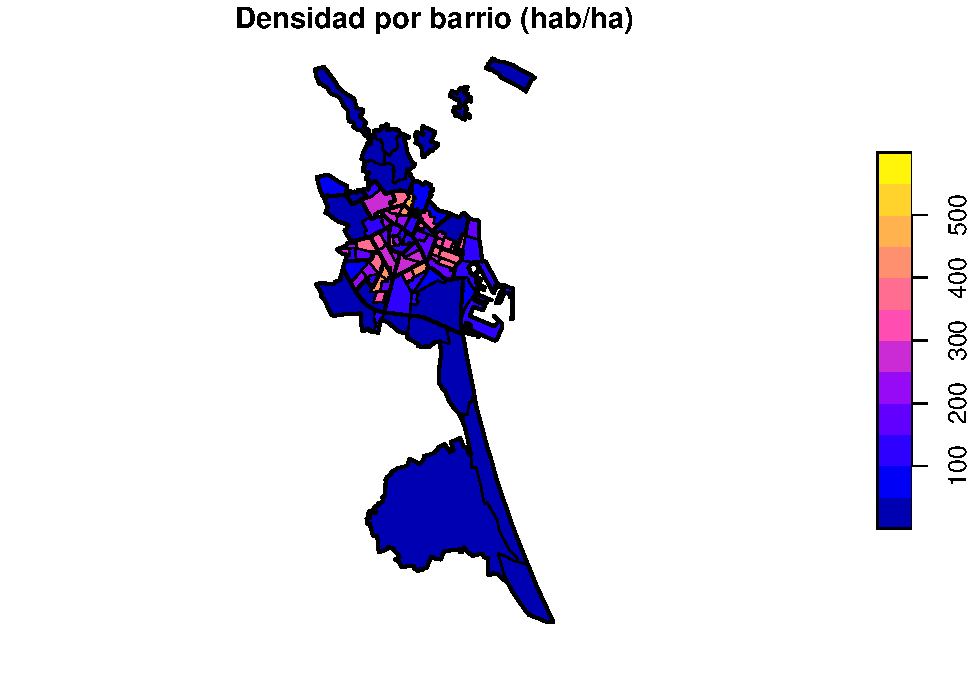
\includegraphics[keepaspectratio]{ProyectoAED_files/figure-latex/unnamed-chunk-9-1.pdf}}

\section{Results}\label{results}

This section may be divided by subheadings. It should provide a concise
and precise description of the experimental results, their
interpretation as well as the experimental conclusions that can be
drawn.

\subsection{Subsection Heading Here}\label{subsection-heading-here}

Subsection text here.

\subsubsection{Subsubsection Heading
Here}\label{subsubsection-heading-here}

Bulleted lists look like this:

\begin{itemize}
\tightlist
\item
  First bullet
\item
  Second bullet
\item
  Third bullet
\end{itemize}

Numbered lists can be added as follows:

\begin{enumerate}
\def\labelenumi{\arabic{enumi}.}
\tightlist
\item
  First item
\item
  Second item
\item
  Third item
\end{enumerate}

The text continues here.

\subsection{Figures, Tables and
Schemes}\label{figures-tables-and-schemes}

All figures and tables should be cited in the main text as Figure
\ref{fig:fig1}, \ref{tab:tab1}, etc. To get cross-reference to figure
generated by R chunks include the
\texttt{\textbackslash{}\textbackslash{}label\{\}} tag in the
\texttt{fig.cap} attribute of the R chunk:
\texttt{fig.cap\ =\ "Fancy\ Caption\textbackslash{}\textbackslash{}label\{fig:plot\}"}.

\begin{figure}
\centering
\pandocbounded{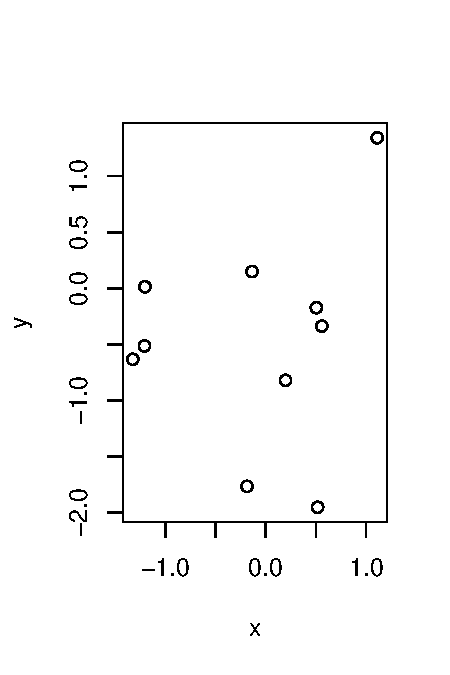
\includegraphics[keepaspectratio,alt={A figure added with a code chunk.}]{ProyectoAED_files/figure-latex/fig1-1.pdf}}
\caption{A figure added with a code chunk.\label{fig:fig1}}
\end{figure}

When making tables using \texttt{kable}, it is suggested to use the
\texttt{format="latex"} and \texttt{tabl.envir="table"} arguments to
ensure table numbering and compatibility with the mdpi document class.

\begin{table}[H]

\caption{\label{tab:tab1}This is a table caption. Tables should be placed in the 
             main text near to the first time they are\textasciitilde{}cited.}
\begin{tabular}[t]{lccc}
\toprule
  & mpg & cyl & disp\\
\midrule
Mazda RX4 & 21.0 & 6 & 160\\
Mazda RX4 Wag & 21.0 & 6 & 160\\
Datsun 710 & 22.8 & 4 & 108\\
Hornet 4 Drive & 21.4 & 6 & 258\\
Hornet Sportabout & 18.7 & 8 & 360\\
\bottomrule
\end{tabular}
\end{table}

For a very wide table, landscape layouts are allowed.

\startlandscape

\begin{table}[H]

\caption{\label{tab:tab2}This is a very wide table}
\begin{tabular}[t]{cccc}
\toprule
Title.1 & Title.2 & Title.3 & Title.4\\
\midrule
Entry 1 & Data & Data & This cell has some longer content that runs over
                               two lines\\
Entry 2 & Data & Data & Data\\
\bottomrule
\end{tabular}
\end{table}

\finishlandscape

\subsection{Formatting of Mathematical
Components}\label{formatting-of-mathematical-components}

This is an example of an equation:

\[
a = 1.
\]

If you want numbered equations use Latex and wrap in the equation
environment:

\begin{equation}
a = 1,
\end{equation}

the text following an equation need not be a new paragraph. Please
punctuate equations as regular text.

This is the example 2 of equation:

\begin{adjustwidth}{-\extralength}{0cm}
\begin{equation}
a = b + c + d + e + f + g + h + i + j + k + l + m + n + o + p + q + r + s + t + 
u + v + w + x + y + z
\end{equation}
\end{adjustwidth}

Theorem-type environments (including propositions, lemmas, corollaries
etc.) can be formatted as follows:

Example of a theorem:

\begin{Theorem}
Example text of a theorem

\end{Theorem}

The text continues here. Proofs must be formatted as follows:

Example of a proof:

\begin{proof}[Proof of Theorem1]
Text of the proof. Note that the phrase ``of Theorem 1'\,' is optional
if it is clear which theorem is being referred to.

\end{proof}

The text continues here.

\section{Discussion}\label{discussion}

Authors should discuss the results and how they can be interpreted in
perspective of previous studies and of the working hypotheses. The
findings and their implications should be discussed in the broadest
context possible. Future research directions may also be highlighted.

\section{Conclusion}\label{conclusion}

This section is not mandatory, but can be added to the manuscript if the
discussion is unusually long or complex.

\section{Patents}\label{patents}

This section is not mandatory, but may be added if there are patents
resulting from the work reported in this manuscript.

\section{Anexo: Información de la
sesión}\label{anexo-informaciuxf3n-de-la-sesiuxf3n}

\begin{Shaded}
\begin{Highlighting}[]
\FunctionTok{sessionInfo}\NormalTok{()}
\end{Highlighting}
\end{Shaded}

\begin{verbatim}
## R version 4.6.1 (2026-06-24)
## Platform: aarch64-apple-darwin23
## Running under: macOS Sonoma 14.7.3
## 
## Matrix products: default
## BLAS:   /Library/Frameworks/R.framework/Versions/4.6/Resources/lib/libRblas.0.dylib 
## LAPACK: /Library/Frameworks/R.framework/Versions/4.6/Resources/lib/libRlapack.dylib;  LAPACK version 3.12.1
## 
## locale:
## [1] en_US.UTF-8/en_US.UTF-8/en_US.UTF-8/C/en_US.UTF-8/en_US.UTF-8
## 
## time zone: Europe/Madrid
## tzcode source: internal
## 
## attached base packages:
## [1] stats     graphics  grDevices utils     datasets  methods   base     
## 
## other attached packages:
##  [1] readxl_1.5.0.1  knitr_1.52      lubridate_1.9.5 forcats_1.0.1  
##  [5] stringr_1.6.0   dplyr_1.2.1     purrr_1.2.2     readr_2.2.0    
##  [9] tidyr_1.3.2     tibble_3.3.1    ggplot2_4.0.3   tidyverse_2.0.0
## [13] sf_1.1-3       
## 
## loaded via a namespace (and not attached):
##  [1] s2_1.1.13          utf8_1.2.6         generics_0.1.4     class_7.3-23      
##  [5] KernSmooth_2.23-26 stringi_1.8.9      hms_1.1.4          digest_0.6.39     
##  [9] magrittr_2.0.5     evaluate_1.0.5     grid_4.6.1         timechange_0.4.0  
## [13] RColorBrewer_1.1-3 fastmap_1.2.0      cellranger_1.1.0   e1071_1.7-17      
## [17] DBI_1.3.0          scales_1.4.0       cli_3.6.6          rlang_1.3.0       
## [21] units_1.0-1        withr_3.0.3        yaml_2.3.12        otel_0.2.0        
## [25] tools_4.6.1        tzdb_0.5.0         vctrs_0.7.3        R6_2.6.1          
## [29] proxy_0.4-29       lifecycle_1.0.5    classInt_0.4-11    rticles_0.27      
## [33] pkgconfig_2.0.3    pillar_1.11.1      gtable_0.3.6       glue_1.8.1        
## [37] Rcpp_1.1.2         xfun_0.61          tidyselect_1.2.1   rstudioapi_0.19.0 
## [41] farver_2.1.2       htmltools_0.5.9    rmarkdown_2.32     wk_0.9.5          
## [45] compiler_4.6.1     S7_0.2.2
\end{verbatim}

%%%%%%%%%%%%%%%%%%%%%%%%%%%%%%%%%%%%%%%%%%

\vspace{6pt}

%%%%%%%%%%%%%%%%%%%%%%%%%%%%%%%%%%%%%%%%%%
%% optional
\supplementary{The following supporting information can be downloaded
at:\\
\linksupplementary{s1}, Figure S1: title; Table S1: title; Video S1:
title.}

% Only for the journal Methods and Protocols:
% If you wish to submit a video article, please do so with any other supplementary material.
% \supplementary{The following supporting information can be downloaded at: \linksupplementary{s1}, Figure S1: title; Table S1: title; Video S1: title. A supporting video article is available at doi: link.}

%%%%%%%%%%%%%%%%%%%%%%%%%%%%%%%%%%%%%%%%%%
\authorcontributions{For research articles with several authors, a short
paragraph specifying their individual contributions must be provided.
The following statements should be used ``X.X. and Y.Y. conceive and
designed the experiments; X.X. performed the experiments; X.X. and Y.Y.
analyzed the data; W.W. contributed reagents/materials/analysis tools;
Y.Y. wrote the paper.'\,' Authorship must be limited to those who have
contributed substantially to the work reported.}

\funding{was funded by NAME OF FUNDER grant number XXX.'\,' and and
\texttt{The\ APC\ was\ funded\ \ by\ XXX\textquotesingle{}\textquotesingle{}.\ Check\ carefully\ that\ the\ details\ given\ are\ accurate\ and\ use\ the\ \ standard\ spelling\ of\ funding\ agency\ names\ at\ \ funding.\ Please\ add:}This
research received no external funding'\,' or ``This research
\url{https://search.crossref.org/funding}, any errors may affect your
future}

\institutionalreview{In this section, you should add the Institutional
Review Board Statement and approval number, if relevant to your study.
You might choose to exclude this statement if the study did not require
ethical approval. Please note that the Editorial Office might ask you
for further information. Please add ``The study was conducted in
accordance with the Declaration of Helsinki, and approved by the
Institutional Review Board (or Ethics Committee) of NAME OF INSTITUTE
(protocol code XXX and date of approval).'' for studies involving
humans. OR ``The animal study protocol was approved by the Institutional
Review Board (or Ethics Committee) of NAME OF INSTITUTE (protocol code
XXX and date of approval).'' for studies involving animals. OR ``Ethical
review and approval were waived for this study due to REASON (please
provide a detailed justification).'' OR ``Not applicable'' for studies
not involving humans or animals.}

\informedconsent{Any research article describing a study involving
humans should contain this statement. Please add
\texttt{Informed\ consent\ was\ obtained\ from\ all\ subjects\ \ involved\ in\ the\ study.\textquotesingle{}\textquotesingle{}\ OR}Patient
consent was waived due to REASON (please provide a detailed
justification).'\,' OR
\texttt{Not\ applicable\textquotesingle{}\textquotesingle{}\ for\ \ studies\ not\ involving\ humans.\ You\ might\ also\ choose\ to\ exclude\ this\ statement\ \ if\ the\ study\ did\ not\ involve\ humans.\ Written\ informed\ consent\ for\ publication\ must\ be\ obtained\ from\ participating\ \ patients\ who\ can\ be\ identified\ (including\ by\ the\ patients\ themselves).\ Please\ \ state}Written
informed consent has been obtained from the patient(s) to publish this
paper'\,' if applicable.}

\dataavailability{We encourage all authors of articles published in MDPI
journals to share their research data. In this section, please provide
details regarding where data supporting reported results can be found,
including links to publicly archived datasets analyzed or generated
during the study. Where no new data were created, or where data is
unavailable due to privacy or ethical re-strictions, a statement is
still required. Suggested Data Availability Statements are available in
section ``MDPI Research Data Policies'' at
\url{https://www.mdpi.com/ethics}.}

\acknowledgments{All sources of funding of the study should be
disclosed. Please clearly indicate grants that you have received in
support of your research work. Clearly state if you received funds for
covering the costs to publish in open access.}

\conflictsofinterest{Declare conflicts of interest or state `The authors
declare no conflict of interest.' Authors must identify and declare any
personal circumstances or interest that may be perceived as
inappropriately influencing the representation or interpretation of
reported research results. Any role of the funding sponsors in the
design of the study; in the collection, analyses or interpretation of
data in the writing of the manuscript, or in the decision to publish the
results must be declared in this section. If there is no role, please
state `The founding sponsors had no role in the design of the study; in
the collection, analyses, or interpretation of data; in the writing of
the manuscript, an in the decision to publish the results'.}

%%%%%%%%%%%%%%%%%%%%%%%%%%%%%%%%%%%%%%%%%%
%% Optional
\sampleavailability{Samples of the compounds \ldots\ldots{} are
available from the authors.}

%% Only for journal Encyclopedia

\abbreviations{Abbreviations}{
The following abbreviations are used in this manuscript:\\

\noindent
\begin{tabular}{@{}ll}
MDPI & Multidisciplinary Digital Publishing Institute \\
DOAJ & Directory of open access journals \\
TLA & Three letter acronym \\
LD & linear dichroism \\
\end{tabular}}

%%%%%%%%%%%%%%%%%%%%%%%%%%%%%%%%%%%%%%%%%%
%% Optional
\input{"appendix.tex"}
%%%%%%%%%%%%%%%%%%%%%%%%%%%%%%%%%%%%%%%%%%
\begin{adjustwidth}{-\extralength}{0cm}

%\printendnotes[custom] % Un-comment to print a list of endnotes


\reftitle{References}
\bibliography{mybibfile.bib}

% If authors have biography, please use the format below
%\section*{Short Biography of Authors}
%\bio
%{\raisebox{-0.35cm}{\includegraphics[width=3.5cm,height=5.3cm,clip,keepaspectratio]{Definitions/author1.pdf}}}
%{\textbf{Firstname Lastname} Biography of first author}
%
%\bio
%{\raisebox{-0.35cm}{\includegraphics[width=3.5cm,height=5.3cm,clip,keepaspectratio]{Definitions/author2.jpg}}}
%{\textbf{Firstname Lastname} Biography of second author}

%%%%%%%%%%%%%%%%%%%%%%%%%%%%%%%%%%%%%%%%%%
%% for journal Sci
%\reviewreports{\\
%Reviewer 1 comments and authors’ response\\
%Reviewer 2 comments and authors’ response\\
%Reviewer 3 comments and authors’ response
%}
%%%%%%%%%%%%%%%%%%%%%%%%%%%%%%%%%%%%%%%%%%
\PublishersNote{}
\end{adjustwidth}


\end{document}
